\documentclass[11pt]{article}

\usepackage[a4paper]{geometry}
\geometry{left=2.0cm,right=2.0cm,top=2.5cm,bottom=2.5cm}

% Chinese support
\usepackage{ctex}

% Math packages
\usepackage{amsmath,amsfonts,amssymb,amsthm,bm,mathrsfs,mathtools,breqn}

% Graphics and Colors
\usepackage{graphicx}
\usepackage{xcolor}
\usepackage{tikz}
\usetikzlibrary{arrows.meta,positioning}
\usepackage{pgfplots}
\pgfplotsset{compat=1.18}
\usepackage{circuitikz}
\graphicspath{{fig/}}

% Units
\usepackage{siunitx}

% Algorithms
\usepackage{algorithm}
\usepackage[noend]{algpseudocode}

% Layout and formatting
\usepackage{fancyhdr}
\usepackage[framemethod=TikZ]{mdframed}
\usepackage{fontspec}
\usepackage{fontsize}
\usepackage{adjustbox}
\usepackage{float}
\usepackage{multicol}
\usepackage{multirow}
\usepackage{pdfpages}
\usepackage{wrapfig}
\usepackage{subcaption}
\usepackage[inline]{enumitem}

% Tables
\usepackage{booktabs}
\usepackage{bigstrut,rotating}

% Listings
\RequirePackage{listings}

% Hyperlinks
\usepackage{hyperref}
\hypersetup{colorlinks=true,linkcolor=blue}

% Cross-referencing
\usepackage[capitalize]{cleveref}
\Crefname{section}{Section}{Sections}
\Crefname{table}{Table}{Tables}
\crefname{table}{Table.}{Tabs.}

% Listing settings
\definecolor{dkgreen}{rgb}{0,0.6,0}
\definecolor{gray}{rgb}{0.5,0.5,0.5}
\definecolor{mauve}{rgb}{0.58,0,0.82}

\lstset{
  frame=tb,
  aboveskip=3mm,
  belowskip=3mm,
  showstringspaces=false,
  columns=flexible,
  framerule=1pt,
  rulecolor=\color{gray!35},
  backgroundcolor=\color{gray!5},
  basicstyle={\small\ttfamily},
  numbers=none,
  numberstyle=\tiny\color{gray},
  keywordstyle=\color{blue},
  commentstyle=\color{dkgreen},
  stringstyle=\color{mauve},
  breaklines=true,
  breakatwhitespace=true,
  tabsize=3,
}

\setmainfont{Palatino Linotype}
\setCJKmainfont{SimSun}[BoldFont=SimHei, ItalicFont=KaiTi]
\setCJKsansfont{SimHei}
\setCJKmonofont{FangSong}
\punctstyle{kaiming}
% 偏好的几个字体, 可以根据需要自行加入字体ttf文件并调用

% Restore standard emphasis to avoid requiring an undefined environment (kaishu).
% The original redefinition used an environment `kaishu` which is not defined
% in a default ctex setup and causes compilation errors. Use \textit for
% emphasis which works across engines.
\renewcommand{\emph}[1]{\textit{#1}}

%改这里可以修改实验报告表头的信息
\newcommand{\experiName}{椭偏法测定介质薄膜厚度和折射率}
\newcommand{\supervisor}{葛琛}
\newcommand{\name}{邓思豪}
\newcommand{\studentNum}{2023K8009909008}
\newcommand{\class}{3}
\newcommand{\group}{01}
\newcommand{\seat}{5}
\newcommand{\dateYear}{2026}
\newcommand{\dateMonth}{4}
\newcommand{\dateDay}{20}
\newcommand{\room}{西实201}
\newcommand{\others}{$\square$}


\begin{document}



\begin{center}
    \LARGE \bf 《\, 基\, 础\, 物\, 理\, 实\, 验\, 》\, 实\, 验\, 报\, 告
\end{center}

\begin{center}
    \noindent \emph{实验名称}\underline{\makebox[25em][c]{\experiName}}
    \emph{指导教师}\underline{\makebox[8em][c]{\supervisor}}\\
    \emph{姓名}\underline{\makebox[6em][c]{\name}} 
    % 如果名字比较长, 可以修改box的长度"6em"
    \emph{学号}\underline{\makebox[10em][c]{\studentNum}}
    \emph{分班分组及座号} \underline{\makebox[5em][c]{\class \ -\ \group \ -\ \seat }\emph{号}} （\emph{例}:\, 1\,-\,04\,-\,5\emph{号}）\\
    \emph{实验日期} \underline{\makebox[3em][c]{\dateYear}}\emph{年}
    \underline{\makebox[2em][c]{\dateMonth}}\emph{月}
    \underline{\makebox[2em][c]{\dateDay}}\emph{日}
    \emph{实验地点}\underline{{\makebox[6em][c]\room}}
    \emph{调课/补课} \underline{\makebox[3em][c]{\others\ 是}}
    \emph{成绩评定} \underline{\hspace{5em}}
    {\noindent}
    \rule[8pt]{17cm}{0.2em}
\end{center}

\section{实验目的}
\begin{enumerate}
    \item 了解薄膜厚度及其折射率等光学参数在近代光学系统中的重要性，认识薄膜参数测量的工程与科研意义。
    \item 掌握椭偏光法（Ellipsometry）的基本原理，包括菲涅耳反射公式、偏振光的反射规律以及等幅椭圆偏振光的获取方法。
    \item 学习并掌握简易椭偏仪（EX1、EX2系列）的内部结构、光路排布及各光学元件（如起偏器、1/4波片、检偏器）的具体物理作用。
    \item 熟练掌握椭偏仪的调试与使用方法，包括入射角/出射角的设定、样品台的俯仰与高度调节、消光点的精确寻找等光学实验基本技能。
    \item 实际测量硅基底上的二氧化硅（$\text{SiO}_2$）薄膜样品的参数，通过消光法获取椭偏参数 $\psi$ 和 $\Delta$。
    \item 掌握使用相关计算软件进行数据分析与理论模型拟合，最终精确测定介质薄膜的厚度 $d$ 和折射率 $n_1$。
\end{enumerate}

\section{实验仪器与用具}
本实验主要使用的仪器与设备包括：
\begin{itemize}
    \item \textbf{椭圆偏振仪主机}（EX1 或 EX2 系列）：包括带有刻度的起偏臂与检偏臂、支撑立板部和底部箱体等，用于实现高精度的角度调节和光路固定。
    \item \textbf{光源系统}：He-Ne 激光器，用于输出波长稳定、方向性好的高纯度单色光束（通常带有红色指示灯以便观察）。
    \item \textbf{偏振与相位调制元件}：
    \begin{itemize}
        \item \textbf{起偏器（Polarizer）}：将光源发出的光转换为具有特定方位角 $P$ 的线偏振光。
        \item \textbf{1/4 波片}：快轴固定在 $+45^\circ$ 位置，使线偏振光产生 $\pi/2$ 的相位延迟，从而获得等幅椭圆偏振光。
        \item \textbf{检偏器（Analyzer）}：用于分析经样品反射后的偏振光状态，通过调节其方位角 $A$ 来寻找光强的极小值（消光点）。
    \end{itemize}
    \item \textbf{光电探测系统}：包含光电倍增管或高灵敏探测器及增益调节旋钮，用于在消光位置附近精确检测极其微弱的光强变化。
    \item \textbf{精密样品台组件}：具有 Z 轴高低调节和二维俯仰调节功能的精密位移台，确保样品表面精确处于入射面内且掠射光线均匀。
    \item \textbf{数据处理与控制设备}：计算机及配套的椭偏数据分析软件（如 ETEX 软件），用于数据的自动采集、模型构建及薄膜参数拟合（使 MSE 达到 $10^{-3}$ 量级）。
    \item \textbf{实验耗材}：待测样品（如硅基底二氧化硅纳米薄膜）及用于夹取样品的专用防污染镊子。
\end{itemize}

\section{实验原理}
椭偏光法测薄膜厚度和折射率的基本思想是：让一束椭圆偏振光以一定的入射角入射到薄膜系统的表面时，光要在单层薄膜的上下表面发生多次折射和反射，在反射方向，反射光束的偏振状态（振幅和相位）会发生变化，而这种变化与薄膜的厚度和折射率有关，因此只要能测量出偏振状态的变化量，就能同时定出膜厚和折射率。如选用特定的条件，又可使测量的计算方法得到简化。

\subsection{理论分析}
薄膜折射率和厚度的测量可归结为反射系数比的测量。
假设玻璃衬底上覆盖有厚度为 $d$ 折射率为 $n_1$ 的均匀透明各向同性的平行平面薄膜系统。一束波长为 $\lambda$ 的单色光，以入射角 $\varphi$ 入射到空气与介质薄膜的界面（I）处，分解为反射和透射两部分，透射部分再与界面（II）相遇，又被分解为反射和透射两部分，这样总的反射光应该是由薄膜系统的两个界面多次反射和折射的光束的叠加而成。

\begin{figure}[H]
    \centering
    
\includegraphics[width=0.6\textwidth]{Figure/fig1.png}
    \caption{各向同性薄膜系统的光反射和折射示意图}
\end{figure}

交界面（I）处 P 和 S 分量的振幅菲涅耳反射比为
\begin{align}
r_{1p} &= \frac{n_1 \cos\varphi - n_0 \cos\varphi_1}{n_1 \cos\varphi + n_0 \cos\varphi_1} \\
r_{1s} &= \frac{n_0 \cos\varphi - n_1 \cos\varphi_1}{n_0 \cos\varphi + n_1 \cos\varphi_1}
\end{align}
在交界（II）处的菲涅耳反射比为
\begin{align}
r_{2p} &= \frac{n_2 \cos\varphi_1 - n_1 \cos\varphi_2}{n_2 \cos\varphi_1 + n_1 \cos\varphi_2} \\
r_{2s} &= \frac{n_1 \cos\varphi_1 - n_2 \cos\varphi_2}{n_1 \cos\varphi_1 + n_2 \cos\varphi_2}
\end{align}
由膜上反射的两相邻光束的相位差为
\begin{equation}
\delta = \frac{4\pi d}{\lambda} n_1 \cos\varphi_1 = \frac{4\pi d}{\lambda} \sqrt{n_1^2 - \sin^2\varphi}
\end{equation}
薄膜系统的总反射比为 $R_p = \frac{(E_p)_r}{(E_p)_i}$ 和 $R_s = \frac{(E_s)_r}{(E_s)_i}$。
经过推导可以得到：
\begin{align}
R_p &= \frac{r_{1p} + r_{2p} \exp(-i\delta)}{1 + r_{1p} r_{2p} \exp(-i\delta)} \\
R_s &= \frac{r_{1s} + r_{2s} \exp(-i\delta)}{1 + r_{1s} r_{2s} \exp(-i\delta)}
\end{align}
薄膜光学常数的测量实则反射比的测量，定义如下：
\begin{equation}
\frac{R_p}{R_s} = \frac{|(E_p)_r| / |(E_s)_r|}{|(E_p)_i| / |(E_s)_i|} \exp[i(\beta_r - \beta_i)]
\end{equation}
在椭偏光法测量中，通常采用椭偏参数 $\psi$ 和 $\Delta$ 来描述反射光的偏振状态的变化，其定义如下：
\begin{align}
\tan\psi &= \frac{|(E_p)_r| / |(E_s)_r|}{|(E_p)_i| / |(E_s)_i|} \\
\Delta &= (\beta_p - \beta_s)_r - (\beta_p - \beta_s)_i = \beta_r - \beta_i
\end{align}
则有
\begin{equation}
\frac{R_p}{R_s} = \tan\psi \exp(i\Delta)
\end{equation}
由前式可知
\begin{equation}
\tan\psi \exp(i\Delta) = \frac{r_{1p} + r_{2p} \exp(-i\delta)}{r_{1s} + r_{2s} \exp(-i\delta)} \cdot \frac{1 + r_{1s} r_{2s} \exp(-i\delta)}{1 + r_{1p} r_{2p} \exp(-i\delta)} = f(n_0, n_1, n_2, \varphi, d, \lambda)
\end{equation}
此式称为椭圆偏振方程。如果入射光的波长和入射角都是确定的，衬底材料的折射率是已知的，则（$\psi$，$\Delta$）就只与 $d$，$n_1$ 有关。在实验前先用计算机进行数值计算，然后再根据测量得到的 $\psi$ 和 $\Delta$ 查表求出 $d$ 和 $n_1$。

\subsection{实验方法}
一种最简单的方法是使入射光在入射处是等幅椭圆偏振光，而在反射处的反射光为线偏振光，在此条件下，$\tan\psi = |(E_p)_r / (E_s)_r| = |\tan A|$，$A$ 即为反射光线偏振光的方位角。
$\Delta = 0$ 或 $\pi \pm (2P - \pi/2)$，$P$ 为获得等幅椭圆偏振光之前的线偏振光的方位角（起偏角）。这样，测量 $\psi$，$\Delta$ 就变成了测量 $A$ 角和 $P$ 角。

\begin{figure}[H]
    \centering
    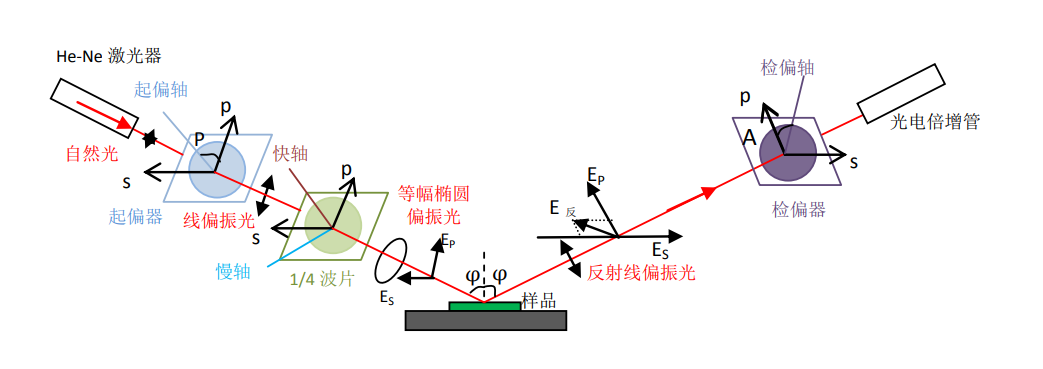
\includegraphics[width=0.8\textwidth]{Figure/fig2.png}
    \caption{椭圆偏振仪基本结构和光路示意图}
\end{figure}

\begin{figure}[H]
    \centering
    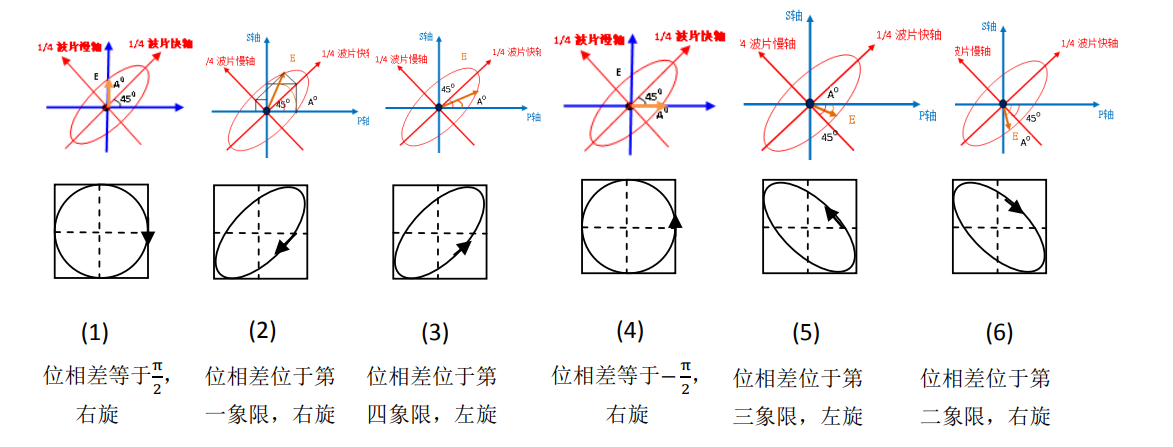
\includegraphics[width=0.8\textwidth]{Figure/fig3.png}
    \caption{椭圆偏振光的获得（1）}
\end{figure}

\begin{figure}[H]
    \centering
    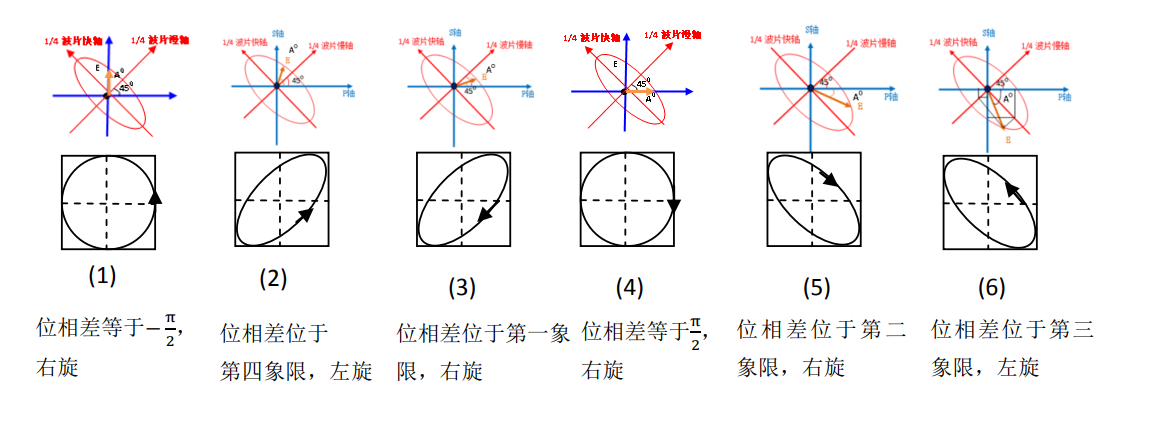
\includegraphics[width=0.8\textwidth]{Figure/fig4.png}
    \caption{椭圆偏振光的获得（2）}
\end{figure}

测量消光点时：
调整起偏器的方位角 $P$，使经过样品反射的光为线偏振光。然后调整检偏器的方位角 $A$，使其主轴与线偏振光的电矢量垂直，处于消光状态，此时光电探测器光电流最小。这样测 $P$ 可确定 $\Delta$，测 $A$ 可确定 $\psi$。

\begin{figure}[H]
    \centering
    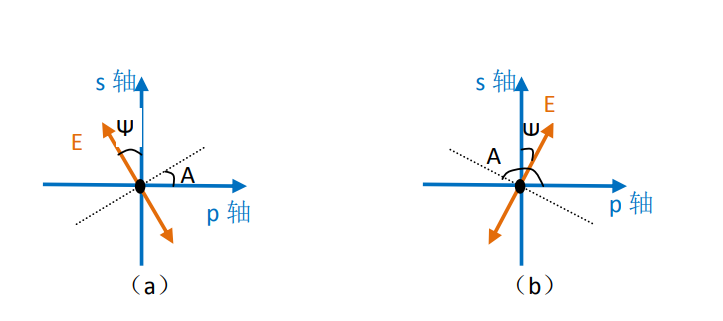
\includegraphics[width=0.6\textwidth]{Figure/fig5.png}
    \caption{检偏器主轴与 P 轴夹角A}
\end{figure}

第一组数据（$A_1$, $P_1$）：
\begin{align}
\psi &= A_1 \\
\Delta &= \pi - \left(2P_1 - \frac{\pi}{2}\right) = \frac{3\pi}{2} - 2P_1
\end{align}
第二组数据（$A_2$, $P_2$）：
\begin{align}
\psi &= A_2 \\
\Delta &= 0 - \left(2P_2 - \frac{\pi}{2}\right) = \frac{\pi}{2} - 2P_2
\end{align}
显然（$A_1$, $P_1$）与（$A_2$, $P_2$）有下列转换关系：
\begin{align}
A_1 + A_2 &= \pi \\
P_1 &= \frac{\pi}{2} + P_2
\end{align}
由这两组数据求出（$\psi$，$\Delta$）后，就可由计算机计算或查表求出膜厚 $d$ 和折射率 $n_1$。

\section{实验内容}
\begin{enumerate}
    \item \textbf{熟悉并掌握椭偏仪的构成}：了解仪器的各部件的作用并学会正确调整。
    \begin{figure}[H]
        \centering
        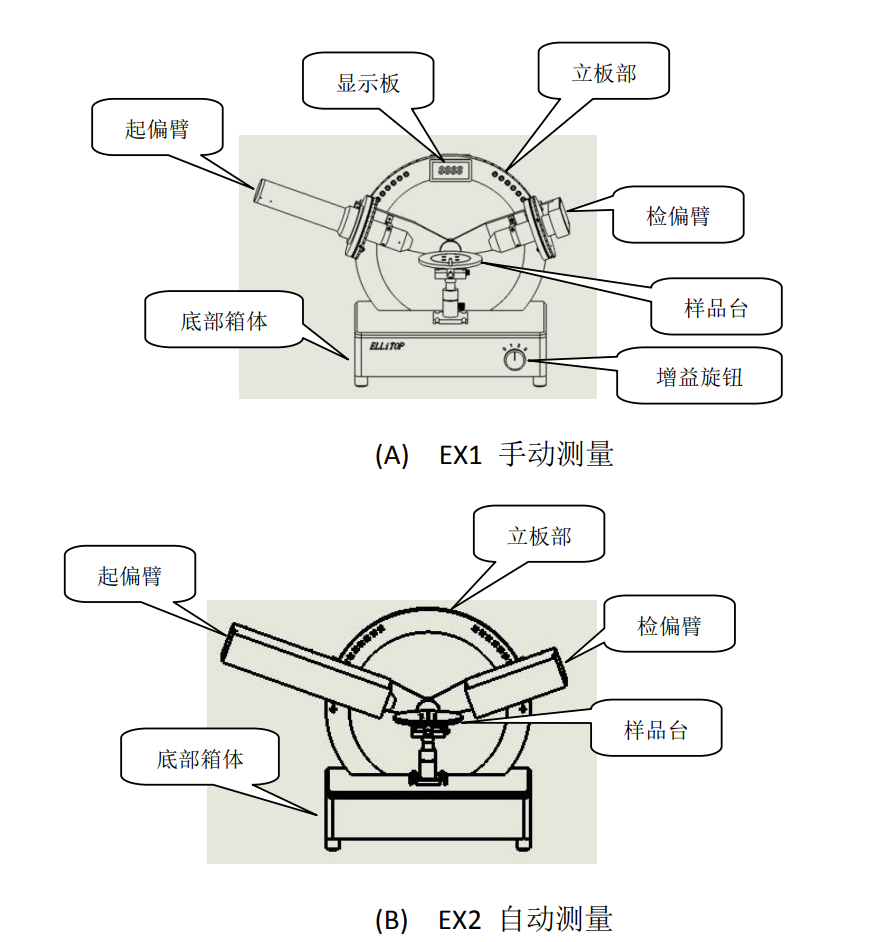
\includegraphics[width=0.6\textwidth]{Figure/fig6.png}
        \caption{EX 系列椭偏仪的主体结构}
    \end{figure}
    \item \textbf{仪器开机预热}：打开电源开关，正常开机后预热30分钟。注意避免身体直接接触激光光束。
    \item \textbf{确定所测样品的入射角度}：保证起偏臂与检偏臂所设置的角度相同。对于Si基底纳米薄膜样品一般选择在$70^\circ$测量。
    \item \textbf{设定入射角和出射角}：拔出定位销，转动起偏臂和检偏臂到目标孔位，并重新锁定。
    \item \textbf{样品的放置和调整}：
    \begin{figure}[H]
        \centering
        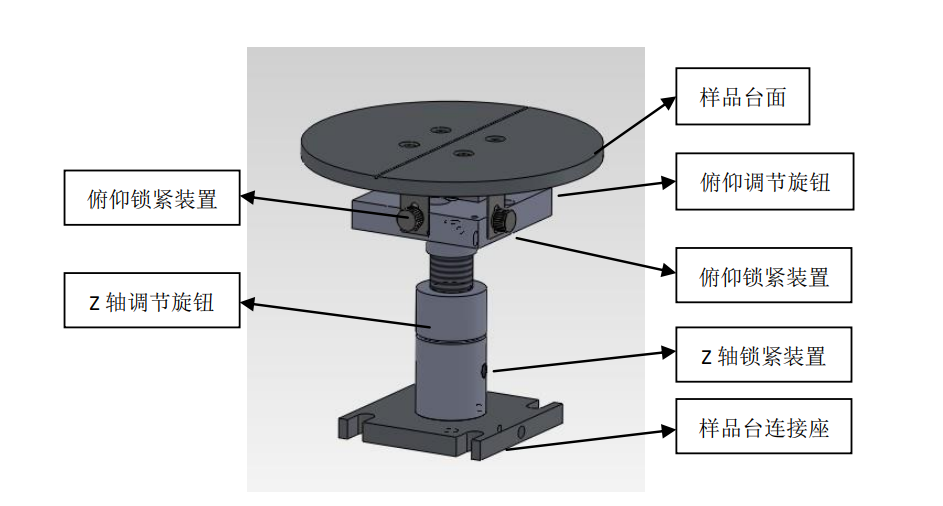
\includegraphics[width=0.6\textwidth]{Figure/fig7.png}
        \caption{样品台结构图}
    \end{figure}
    \begin{itemize}
        \item 将样品放置于样品台面。
        \item 调节起偏臂至$90^\circ$。调节样品台高低和俯仰，使入射光掠射样品表面，亮线均匀。
        \item 将起偏臂角度调至待测角度，精调俯仰旋钮使反射光进入检偏臂光阑中心，直到探测器光强最大。
    \end{itemize}
    \item \textbf{测量纳米薄膜的膜厚 $d$ 和折射率 $n_1$}：
    \begin{itemize}
        \item 测量消光点$(P_1, A_1)$和$(P_2, A_2)$。
        \item 计算椭偏角$(\psi, \Delta)$。
        \item 利用计算机软件进行数据分析和查表拟合，求出 $d$ 和 $n_1$。
    \end{itemize}
    \item \textbf{重复测量}：对样品的一个位置测量2遍观察重复性；在3个不同位置重复测量，观测均匀性。
    \item \textbf{误差分析}：对实验结果进行误差分析。
    \item \textbf{仪器关机}：先关闭软件及计算机系统，再关闭仪器电源。
\end{enumerate}

\section{实验数据处理}

本次实验对硅基底二氧化硅薄膜样品的三个不同位置进行了测量，每个位置分别测量两次。测量数据整理如下表所示：

\begin{table}[H]
    \centering
    \caption{椭偏法测量二氧化硅薄膜实验数据表}
    \vspace{0.2cm}
    \begin{tabular}{ccccccc}
        \toprule
        \textbf{测量位置} & \textbf{测量次数} & \textbf{膜厚 $d$ (nm)} & \textbf{折射率 $n_1$} & \textbf{MSE ($10^{-3}$)} & \textbf{平均厚度 (nm)} & \textbf{平均折射率} \\
        \midrule
        \multirow{2}{*}{位置1} & 1 & 113.03 & 1.4889 & 6.60 & \multirow{2}{*}{113.26} & \multirow{2}{*}{1.4878} \\
                               & 2 & 113.48 & 1.4867 & 5.48 & & \\
        \midrule
        \multirow{2}{*}{位置2} & 1 & 110.90 & 1.4973 & 1.36 & \multirow{2}{*}{111.46} & \multirow{2}{*}{1.4910} \\
                               & 2 & 112.02 & 1.4846 & 2.01 & & \\
        \midrule
        \multirow{2}{*}{位置3} & 1 & 112.07 & 1.4860 & 2.64 & \multirow{2}{*}{112.52} & \multirow{2}{*}{1.4842} \\
                               & 2 & 112.97 & 1.4824 & 3.83 & & \\
        \bottomrule
    \end{tabular}
\end{table}

\subsection*{1. 数据计算与不确定度分析}
对上述 6 次测量的膜厚 $d$ 和折射率 $n_1$ 进行统计处理：
\begin{itemize}
    \item \textbf{膜厚 $d$ 的平均值及标准差：}
    \begin{equation}
        \bar{d} = \frac{1}{6} \sum_{i=1}^6 d_i = 112.41 \text{ nm}
    \end{equation}
    实验标准差 $S_d = \sqrt{\frac{\sum (d_i - \bar{d})^2}{6-1}} = 0.937 \text{ nm}$，A类不确定度 $u_A(d) = \frac{S_d}{\sqrt{6}} \approx 0.38 \text{ nm}$。
    最终膜厚测量结果可表示为：
    \begin{equation}
        d = 112.41 \pm 0.38 \text{ nm}
    \end{equation}
    
    \item \textbf{折射率 $n_1$ 的平均值及标准差：}
    \begin{equation}
        \bar{n}_1 = \frac{1}{6} \sum_{i=1}^6 n_{1i} = 1.4877
    \end{equation}
    实验标准差 $S_n = \sqrt{\frac{\sum (n_{1i} - \bar{n}_1)^2}{6-1}} = 0.0052$，A类不确定度 $u_A(n_1) = \frac{S_n}{\sqrt{6}} \approx 0.0021$。
    最终折射率测量结果可表示为：
    \begin{equation}
        n_1 = 1.4877 \pm 0.0021
    \end{equation}
\end{itemize}

\subsection*{2. 实验消光曲线展示}
为了直观展示椭偏仪的消光过程，我们选取了其中一次实验的扫描寻峰数据（对应第一组测量的 details 步骤）绘制了光强百分比随检偏器角度 $A$ 变化的消光曲线，如图 \ref{fig:extinction} 所示。

\begin{figure}[H]
    \centering
    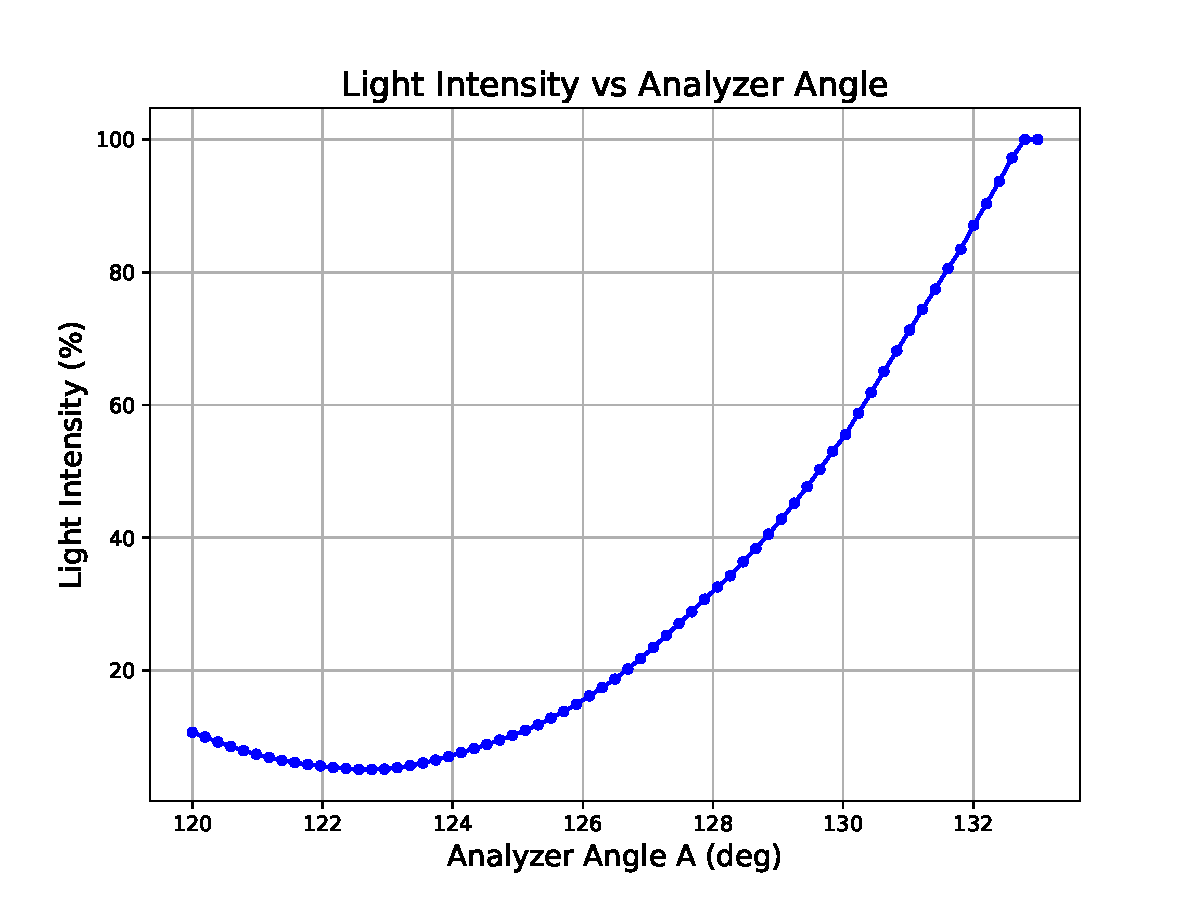
\includegraphics[width=0.7\textwidth]{Figure/extinction_curve.pdf}
    \caption{检偏器角度与光强关系的消光曲线}
    \label{fig:extinction}
\end{figure}

当检偏器角度 $A$ 处于约 $122.75^\circ$ 时，光强出现极小值（约为 5.08\%）。这说明此时经样品反射后的偏振光中，某一特定方向的电矢量分量被检偏器几乎完全阻挡，达到了消光状态。因为经过 $1/4$ 波片调节后入射样品的是等幅椭圆偏振光，样品表面反射后的光变为线偏振光，所以我们可以通过寻找这一光强极小值来准确定位反射线偏振光的偏振方向，进而结合起偏角 $P$ 得到椭偏参数 $\psi$ 与 $\Delta$。

\subsection*{3. 物理意义及结论分析}
结合实验数据，可以得出以下物理结论：
\begin{enumerate}
    \item \textbf{重复性与稳定性：} 在同一位置进行的两次重复测量中，得到的厚度偏差和折射率偏差极小（如位置1的两次测量偏差仅在 $0.45\text{ nm}$ 左右），说明仪器的稳定性好，且实验操作中通过光电探测器寻峰确定的消光点极为精准。同时，测量数据拟合的均方误差（MSE）均在 $10^{-3}$ 量级，表明基于菲涅耳公式建立的椭圆偏振理论模型在此系统下十分适用且可靠。
    \item \textbf{薄膜均匀性分析：} 通过对比样品 3 个不同位置的测量结果可以发现，薄膜厚度在 $110.90\text{ nm}$ 到 $113.48\text{ nm}$ 之间波动。这种约 $2\sim 3\text{ nm}$ 的宏观厚度差异，反映出在半导体镀膜工艺（如热氧化法制备 $\text{SiO}_2$）中，薄膜的生长速率在基底不同区域存在微小的非均匀性，这在工程实际中是常见且合理的。
    \item \textbf{折射率分析：} 测得的薄膜折射率均值为 $1.4877$，与理想非晶态 $\text{SiO}_2$ 在可见光波段的标准折射率（约 $1.45\sim 1.46$）相比略微偏高。从物理机制上分析，这可能是因为实际生长的薄膜内部存在一定的应力，或者是表面吸附了空气中的水分和杂质，导致介电常数发生微小改变，体现了实际材料与理想模型的差异。
\end{enumerate}

\section{思考题}
\begin{enumerate}
    \item 椭偏光法测薄膜厚度和折射率的基本思想是什么？
    
    \textbf{答：}椭偏光法测量薄膜厚度和折射率的基本思想是利用光在薄膜表面反射时偏振状态的变化来推导膜层的光学性质。具体机理如下：
    
    当一束椭圆偏振光以入射角 $\varphi$ 入射到薄膜系统（空气-薄膜-衬底三层结构）的表面时，光在薄膜的上下界面处分别发生菲涅耳反射，所有反射光的矢量合成形成总反射光。根据菲涅耳公式，P分量和S分量的反射系数分别为：
    \begin{align}
        r_p &= \frac{n_1 \cos\varphi - n_0 \cos\varphi_1}{n_1 \cos\varphi + n_0 \cos\varphi_1}, \quad
        r_s = \frac{n_0 \cos\varphi - n_1 \cos\varphi_1}{n_0 \cos\varphi + n_1 \cos\varphi_1}
    \end{align}
    薄膜上下界面反射的两相邻光束间存在相位差 $\delta = \frac{4\pi d}{\lambda}\sqrt{n_1^2 - \sin^2\varphi}$，这个相位差直接关联到膜厚 $d$。通过多光束干涉和相位累积，总的反射系数比为：
    \begin{equation}
        \frac{R_p}{R_s} = \tan\psi \exp(i\Delta)
    \end{equation}
    其中椭偏参数 $\psi$ 和 $\Delta$ 完全由膜厚、折射率、入射角和波长决定。通过实验测得 $\psi$ 和 $\Delta$，结合菲涅耳反射理论进行非线性拟合，即可唯一确定 $d$ 和 $n_1$。这正是椭偏光法的核心：光学参数的变化被精确编码在反射光的偏振态中，使得只需两个参数 $(\psi, \Delta)$ 就能确定两个未知量。
    
    \item 等幅椭圆偏振光是如何获得的，简述其原理。
    
    \textbf{答：}等幅椭圆偏振光的获得涉及两个关键光学元件：起偏器和1/4波片的协作。
    
    \textbf{第一步（起偏器）：}非偏振光或自然光经过起偏器后转换为线偏振光。起偏器作用相当于一个方向选择器，其传轴方向为 $P$（起偏角）。设入射光强度为 $I_0$，则透射光强度为 $I_p = I_0/2$（对于非偏振光），其电矢量在起偏器坐标系中表示为：
    \begin{equation}
        \vec{E}_{线} = E_0(\cos P \, \hat{x} + \sin P \, \hat{y})
    \end{equation}
    
    \textbf{第二步（1/4波片）：}线偏振光入射到1/4波片，快轴固定在 $+45°$ 位置。关键在于线偏振光的电矢量方向相对于波片的快慢轴形成特定角度。当线偏振光与快轴成 $45°$ 夹角时，其在快轴和慢轴上的分量相等：
    \begin{equation}
        E_{快} = E_0 \cos 45° = \frac{E_0}{\sqrt{2}}, \quad E_{慢} = E_0 \sin 45° = \frac{E_0}{\sqrt{2}}
    \end{equation}
    
    波片对这两个分量引入的相位差为 $\Delta\phi = \frac{2\pi}{\lambda}(n_{慢} - n_{快}) d_{波片}$。对于1/4波片，满足 $\Delta\phi = \pi/2$，即在出射端：
    \begin{equation}
        E_{快}' = \frac{E_0}{\sqrt{2}} e^{i\phi_1}, \quad E_{慢}' = \frac{E_0}{\sqrt{2}} e^{i(\phi_1 + \pi/2)}
    \end{equation}
    
    两个分量在空间中形成垂直关系且振幅相等，相位差为 $\pi/2$，这正是**等幅椭圆偏振光**的定义。其参数方程为：
    \begin{equation}
        x = \frac{E_0}{\sqrt{2}} \cos\omega t, \quad y = \frac{E_0}{\sqrt{2}} \sin\omega t
    \end{equation}
    电矢量的端点在时间演化中描绘出一个圆（等幅椭圆退化为圆）。这种等幅椭圆偏振光具有关键性质：当它从样品表面反射后，P分量和S分量的反射系数差异会使其变成线偏振光，便于进行消光测量。
    
    \item $1/4$ 波片的作用是什么？
    
    \textbf{答：}1/4波片是光学相位延迟元件，其核心作用是**引入特定的相位延迟以实现偏振态转换**。
    
    \textbf{物理机制：}双折射材料（如云母、液晶等）具有两个不同的主折射率 $n_{快}$ 和 $n_{慢}$。当光通过该材料时，沿快轴和慢轴方向的光波传播速度不同，导致相位累积速率不同。设波片厚度为 $d$，光在波片中传播距离为 $d$，则两轴上的相位分别为：
    \begin{align}
        \phi_{快} &= \frac{2\pi n_{快}}{\lambda} d \\
        \phi_{慢} &= \frac{2\pi n_{慢}}{\lambda} d
    \end{align}
    相位差为：
    \begin{equation}
        \Delta\phi = (\phi_{慢} - \phi_{快}) = \frac{2\pi (n_{慢} - n_{快})}{\lambda} d = \frac{2\pi \Delta n}{\lambda} d
    \end{equation}
    对于1/4波片，相位差正好为 $\pi/2$（即 $\lambda/4$ 的光程差）：
    \begin{equation}
        \Delta\phi_{1/4} = \frac{\pi}{2} = \frac{2\pi \Delta n}{\lambda} d \quad \Rightarrow \quad d = \frac{\lambda}{4\Delta n}
    \end{equation}
    
    \textbf{在椭偏仪中的应用作用：}
    \begin{enumerate}
        \item \textbf{线偏振光 → 等幅椭圆偏振光}：当线偏振光与快轴成 $45°$ 入射时，通过 $\pi/2$ 的相位延迟，两个正交分量变成相位差为 $90°$ 且振幅相等的状态，形成圆偏振光（等幅椭圆偏振的特例）。
        \item \textbf{编码样品信息}：等幅椭圆偏振光从样品反射后，因菲涅耳反射的波长依赖性，P分量和S分量的反射系数不同，使反射光重新变为线偏振光，这个线偏振光方向蕴含了薄膜的厚度和折射率信息。
        \item \textbf{消光点法的基础}：通过检偏器与反射线偏振光垂直时达到消光状态，1/4波片的 $\pi/2$ 相位延迟确保了该过程高度灵敏，最终使得椭偏参数测量精度达到 $10^{-3}$ 量级。
    \end{enumerate}
    
    因此，1/4波片是椭偏仪的"相位调制器"，其 $\pi/2$ 延迟量经过精确设计，既能生成理想的等幅椭圆入射光，又能通过样品的反射特性使偏振态变化被最大化地放大，是实现高精度椭偏测量的关键光学元件。
\end{enumerate}
\end{document}